\documentclass[a4paper,10pt,oneside,openany]{book}
\usepackage[utf8]{inputenc}
\usepackage{amsmath}
\usepackage{cancel}
\usepackage{amsfonts}
\usepackage{amssymb}
\usepackage{xcolor}
\usepackage{mathrsfs}
\usepackage{amsfonts}
\usepackage{amsmath}
\usepackage{mathtools}
\usepackage{centernot}
\usepackage{graphicx}
\usepackage{setspace}
\usepackage{geometry}
\usepackage{tcolorbox}
\usepackage{hyperref}
\usepackage{stackengine}
%%%%%%%%%%%%%%%%%%%%%%%%%%%%%%%%%%%%%%%%%%%%%%%%%%%%%%%%%%%%%%%%%%%%%%%%%%%%%%%%%%%%%%%%%%%%%%%%%%
\usepackage{multicol}

%%%%%%%%%%%%%%%%%%%%%%%%%%%%%%%%%%%%%%%%%%%%%%%%%%%%%%%%%%%%%%%%%%%%%%%%%%%%%%%%%%%%%%%%%%%%%%%%%%
\usepackage{listings}
\usepackage{color}
\usepackage{qtree}

\definecolor{dkgreen}{rgb}{0,0.6,0}
\definecolor{gray}{rgb}{0.5,0.5,0.5}
\definecolor{mauve}{rgb}{0.58,0,0.82}

\lstset{frame=tb,
  language=C++,
  aboveskip=3mm,
  belowskip=3mm,
  showstringspaces=false,
  columns=flexible,
  basicstyle={\small\ttfamily},
 %numbers=left,
  numbers=none,
  numberstyle=\tiny\color{gray},
  keywordstyle=\color{blue},
  commentstyle=\color{dkgreen},
  stringstyle=\color{mauve},
  breaklines=true,
  breakatwhitespace=true,
  tabsize=3,
  %xleftmargin=0.5cm
}
%%%%%%%%%%%%%%%%%%%%%%%%%%%%%%%%%%%%%%%%%%%%%%%%%%%%%%%%%%
\usepackage{graphicx}
\graphicspath{ {images/} }

\definecolor{grigio}{RGB}{179,179,179}
%\theoremstyle{plain}
\newtheorem{thm}{Teorema}[section]
\newtheorem{deff}{Definizione}[section]
\newtheorem{dimm}{Dimostrazione}[section]

\geometry{a4paper,top=1.5cm,bottom=1.5cm,left=2.5cm,right=2.5cm,%
heightrounded,bindingoffset=5mm}

\newcommand{\tb}[1]{\textbf{#1}}
\newcommand{\e}[1]{\textit{#1}}
\newcommand{\DEF}[1]{\textcolor{blue}{DEF:}}
\newcommand{\om}[0]{$\Omega$}
\newcommand{\al}[0]{$\mathcal{A}$}
\newcommand{\zero}[0]{$\emptyset$}
\newcommand{\ap}[0]{$\in$}
\newcommand{\im}[0]{$\implies$}

\setcounter{tocdepth}{1} %il grado di profondita indice, 1 solo chapter, 2 section ...

\author{Edoardo Lenzi}
\title{LFC (Linguaggi Formali e Compilatori) - Note del Corso}
\begin{document}
\maketitle
\tableofcontents
%\chapter{Introduzione}
Un compilatore \'e un programma che legge un \textbf{linguaggio source} e lo traduce in un \texttt{equilvalente} \textbf{linguaggio di programmazione
target}. 
Solitamente il compilatore compila in \texttt{assembly} e poi un \textbf{assembler} produce codice macchina.
Se il target language \'e un programma eseguibile pu\'o processare input e produrre output.

Un \textbf{interprete} \'e un altro tipo di language processor, invece di tradurre il linguaggio lo esegue direttamente
quindi piglia sia il source program che gli input e processa l'output

Infine il \textbf{preprocessore} risolve le macro nel sorgente codificandole in linguaggio nativo (espandendole) prima di compilare.

\begin{quote}
Solitamente il compilato va pi\'u veloce mentre l`interprete ti da diagnosi piu accurate dato che esegue il codice.
Nel caso di Java compilo il sorgente in linguaggio intermedio \texttt{bytecode} che poi interpreto sulla JVM.
\end{quote}

Il \textbf{linker} \lq\lq linka\rq\rq\ assieme moduli e librerie dove ho riferimenti ad altri file (risolve gli indirizzi).
Il \textbf{loader} invece fa il merge in memoria per l'esecuzione.

%img4

\section{Front-End of the Compiler}
La \textbf{parte analitica} del processo di compilazione spacca la sorgente in parti costituenti e impone su di esse una struttura 
grammaticale (stile dtd); sfrutta questa struttura per creare una rappresentazione intermedia.
Se non passa la validazione grammaticale mi tira errori. Il sorgente viene storicizzato in
una struttura dati chiamata \textbf{symbol table}. 

\section{Back-End of the Compiler}
La \textbf{parte di sintesi} invece traduce il sorgente guardando la rappresentazione intermedia e la symbol table;
le parti di analisi e sintesi sono chiamate anche \textbf{front-end of the copiler} mentre le restanti \textbf{back-end}.

\section{Lexical analysis}
Fa uno scan e raggruppa le parole in \textbf{lexems}, per ogni lexem genera un \textbf{token} della forma

\begin{center}
    \texttt{(token name, attribute value)} 
\end{center}

Il \texttt{token name} \'e un simbolo astratto usato nella syntax analysis
mentre il \texttt{value} \'e un puntatore alla symbol table entry.\\[5pt]

\textbf{ie)}
\begin{quote}
    \texttt{position = initial + rate * 60} diventa \texttt{(id, 1) (=) (id, 2) (+) (id, 3) (*) (60)}\\
    gli operatori matematici sono simboli astratti che non hanno attribute value (?non sono referenziati nella symbol table?).
\end{quote}

%img7

\section{Session syntax analyzer} 
\'E un parsing, con i token crea una \textbf{rappresentazione ad albero (syntax tree)} nel quale 
il nodo \'e un operatore e i figli gli operandi. 

gli operatori devono avere priorit\'a per costruire l'albero, la struttura grammaticale serve anche a 
definire le priorit\'a degli operatori.

\section{Semantic analyzer} 
Piglia il \texttt{syntax tree} e guarda se \'e semanticamente consistente con la definizione del linguaggio.
(ie \texttt{type checking}). Il linguaggio puo ammettere cast impliciti chiamati \textbf{coercizioni} o tirare cogne.

\lq\lq \textit{intofloat}\rq\rq \'e una coercizione dell'intero 60 in float dato che gli altri operandi sono float. 

\section{Intermediate code generation}
Nel processo di compilazione posso avere varie rappresentazioni intermedie come alberi etc..
Dopo semantic analysis solitmente creo un codice basso livello, machine-like, \textit{\lq\lq easy to 
produce and esay to translate int target machine code\rq\rq}. Nella figura ho un tree address code
ricavato dal syntax tree. 

In un tree address code a destra ho al massimo un operatore (assembly like), e le operazioni sono in ordine.

Devo avere variabiline intermedie
\section{Code generation}
Segue la fase opzionale di \textbf{code optimization}, prende la rappresentazione intermedia e la mappa in un target language.
Le istruzioni intermedie vengono tradote in istruzioni macchina (presumibilmente). Devo capire come mappare variabili su registri

Nella symbol table devo storicizzare tutti gli attributi di un variable name.
 
Solitamente posso agglomerare le fasi di analisi in front end pass e le altre in back end pass.







%\chapter{Progetto}
%https://sites.google.com/a/unitn.it/software-engineering-ii---designing-applications-that-matter/home
%https://github.com/marcorobol/is2-2017
%https://www.facebook.com/trentose2
%https://sites.google.com/site/sphoebss/project-definition
%https://sites.google.com/site/disibpm/

DOM struttura della pagina HTML 
JS mono-thread ma si comporta come multithread
devo installare nodeJs (verifico la presenza con \texttt{node -v}

Devo buttare tutto su heroku


%%%%%%%%%%%%%%%%%%%%%%%%%%%%%%%%%%%%%%%%%%%%%%%%%%%%%%%%%%%%%%%%
\chapter{Application Design}
\section{The Design Process}
\subsection{Empathize Mode}
L'empatia \'e lo sforzo nel capire l'utente, le sue abitudini ed i suoi problemi per disegnare un app utile.

\subsection{Define Mode}
Creo un design in base a cosa ho appreso dal contesto umano.

\subsection{Ideate Mode}
La parte del processo in cui mi concentro nella creazione delle nuove idee. 
Vado nel profondo, cerco di definire tutto quello che mi serve per realizzare un mockup.

\subsection{Prototype Mode}
Per vedere qualcosa e risolvere problemi fondamentali di design. \lq\lq Fail early and cheaply!\rq\rq .

\subsection{Test Mode}
Una seconda occasione di confronto con l'utente.

\section{EDD Empathy Driven Design}
Empathy: the feeling that you understand and share another person's experience and emotions. 
The ability to share someone else's feeling.

%%%%%%%%%%%%%%%%%%%%%%%%%%%%%%%%%%%%%%%%%%%%%%%%%%%%%%%%%%%%%%%
\chapter{Agile Development}

\begin{tcolorbox}
	\begin{center}
		Kanban e Scrum
	\end{center}
\end{tcolorbox}

\begin{itemize}
	\item development process\\
	\item principali tipi di processo\\
	\item	processi agile (caratteristiche e pro)\\
	\item Scrum e Kanban (similitudini e differenze)\\
	\item	come definire, caratterizzare ed eseguire:\\
		\item[-] user stories\\
		\item[-] backlogs\\
		\item[-] sprints\\
	\item linkare backlogs a github issues\\
%%%%%%%%%%%%%%%%%%%%%%%%%%%%%%%%%%%%%%%%%%%%%%%%%%%%%%%%%%%%%%%%%%%%%%%%%
https://www.atlassian.com/agile
\section{What is agile}
\'E un approccio iterativo al project management e sw development;
molti piccoli incrementi (consegno il lavoro un pezzo alla volta). 
Tutti i piani, requisiti e risultati vengono rivisti spesso cos\'i da rendere 
il team resistente a cambiamenti in corso d'opera.

Il team si prende il controllo di come fare il lavoro, si autoorganizza per 
portare a termine task granulari.

\'E un set di tecniche di sviluppo accomunate dal continuo processo di 
miglioramento. Il manifesto Agile non da regole precise ma solo valori e 
linee guida che pongono le persone al primo posto.

\section{Il manifesto Agile}
http://agilemanifesto.org/iso/it/manifesto.html
siamo arrivati a considerare importanti:
\begin{itemize}
	\item \textbf{Gli individui e le interazioni} più che i processi e gli strumenti\\
	\item \textbf{Il software funzionante} più che la documentazione esaustiva\\
	\item \textbf{La collaborazione col cliente} più che la negoziazione dei contratti\\
	\item \textbf{Rispondere al cambiamento} più che seguire un piano\\
\end{itemize}

\subsection{I principi}
Seguiamo questi principi:

La nostra massima priorità è soddisfare il cliente
rilasciando software di valore, fin da subito
e in maniera continua.

Accogliamo i cambiamenti nei requisiti,
anche a stadi avanzati dello sviluppo.
I processi agili sfruttano il cambiamento
a favore del vantaggio competitivo del cliente.

Consegnamo frequentemente software funzionante,
con cadenza variabile da un paio di settimane a un paio di mesi,
preferendo i periodi brevi.

Committenti e sviluppatori devono lavorare insieme
quotidianamente per tutta la durata del progetto.

Fondiamo i progetti su individui motivati.
Diamo loro l'ambiente e il supporto di cui hanno bisogno
e confidiamo nella loro capacità di portare il lavoro a termine.

Una conversazione faccia a faccia
è il modo più efficiente e più efficace per comunicare
con il team ed all'interno del team.

Il software funzionante è il principale metro di misura di progresso.

I processi agili promuovono uno sviluppo sostenibile.
Gli sponsor, gli sviluppatori e gli utenti dovrebbero essere in grado
di mantenere indefinitamente un ritmo costante.

La continua attenzione all'eccellenza tecnica
e alla buona progettazione esaltano l'agilità.

La semplicità - l'arte di massimizzare la quantità
di lavoro non svolto - è essenziale.

Le architetture, i requisiti e la progettazione
migliori emergono da team che si auto-organizzano.

A intervalli regolari il team riflette su come
diventare più efficace, dopodiché regola e adatta
il proprio comportamento di conseguenza. 

\section{Aglie Frameworks}
Dal 2001 quando nasce il manifesto sono nati vari frameworks come Scrum, 
Kanban ed Extreme Programming (XP). Accomunati da iterazioni frequenti,
continuo imparare/aggiornarsi. 

\section{Project Management}
Un approccio iterativo per managing sw development projects, focalizzato 
su release continue e feedback continui. Il project management pu\'o essere 
categorizzato attraverso due frameworks: kanban e scrum.

\subsection{Scrum [Mischia]}
Fixed length iterations chiamati sprint.

ha 2 backlogs: 
	product backlog (lavoro che dev'essere fatto), ordinato per priorit\'a 
	sprint backlog, prendo gli issue dal prod backlog finchè la capacit\'a dello 
	sprint \'e saturata.

Nel team ci sono ruoli predefiniti:
	Scrum Master del team 
	Product Owner
	Scrum Team 

\subsection{Le quattro cerimonie}
Sprint Planning, meeting per capire quello che manca per finire lo sprint corrente
Sprint Demo, spiega cosa hanno realizzato nello sprint 
Daily StandUp, meeting di 15 minuti per sincronizzare il team 
Retrospective una review di cosa \'e andato bene e cosa migliorare

\subsection{Scrum Board}
To do, in progress, code review, done

\section{Kanban}
Focalizzato a fare le cose nel minor tempo possibile, mi permette di reagire 
a cambiamenti anche prima di Scrum. Non usa backlogs ma si focalizza solo 
sulla ToDo column questo permette di focalizzarsi su release continue che 
vengono fatte in qualunque momento.

Appena finisco qualcosa lo metto in done, il carico di lavoro sul team 
deve restare sotto il limite del WIP limit (un limite predefinito calcolato 
sulla capacit\'a del team) non posso superare con il lavoro in progress il 
WIP.

\subsection{Kanban four components}
stories (list of work) issues o task da fare
columns of lanes usate nella kanban board per distinguere diversi workstreams, users, projects, etc
Work In Progress limit limite calcolato sulla capacit\'a del team
Continuous Releases, il team lavora sulle stories sotto il limite WIP e pu\'o fare una release in qualsiasi momento.

\section{Estimated, Report and Plan}
Qualsiasi agile framework venga usato, devo visualizzare l'andamento del lavoro 
nel mio team per pianificare i futuri sprint.

In Kanban gli estimate sono molto importanti infatti il WIP si calcola sulle 
precedenti esperienze e team size. In Scrum mi serve per capire quanto lavoro 
posso fare nel prossimo sprint. 

Solitamente ad ogni task viene assegnato un peso per capire numericamente 
quanto ci metto. 
Le estimation vengono in gioco solo all'inizio/fine sprint; gli 
\textbf{agile report} mi da dei parametri del progresso dello sprint corrente 
(burndown charts) [basato sul numero di story points terminati].

\section{Grooming product backlog}
All'inizio di ogni sprint prendo dal backlog gli story points con priorit\'a maggiore,
il backlog \'e fondamentale proprio per avere una visione del progetto in toto, va mantenuto 
aggiornato.
%%%%%%%%%%%%%%%%%%%%%%%%%%%%%%%%%%%%%%%%%%%%%%%%%%%%%%%%%%%%%%%%%%%%%%%%%%%

http://leankit.com/
https://www.pivotaltracker.com/
Book: "Scrum: The Art of Doing Twice the Work in Half the Time"

https://www.proprofs.com/quiz-school/preview.php?title=ODM2MzUxL9VY
Sono in ritardo:
	lavoro extra
	consegno meno
	ritardo consegna (allungo lo sprint)
	allargo il team

Quale non è parte di scrum
	sprint planning meeting
	product review meeting
	sprint retrospective meeting

Principali differenze scrum e kanban 
Fasi del processo Scrum

%%%%%%%%%%%%%%%%%%%%%%%%%%%%%%%%%%%%%%%%%%%%%%%%%%%%%%%%%%%%%%
\chapter{Versioning and Collaboration}
git commands:
	init - how to start an empty repo
	clone
	status
	log
	checkout
	diff
	add - and why we have a staging area, how to use it
	commit - and commit strategies, when it is proper to commit
	merge - and solving merge conflicts
	branch - and when to branch/merge
	pull, push
	remote - setting up a remote repository
	rebase - and why/when to use it
	reset (and reset hard): when and how to revert to a state
	stash
	how/why to fork and perform pull requests

[GIT CLI]
https://www.atlassian.com/git/tutorials/what-is-version-control#benefits-of-version-control

[PR]
https://help.github.com/articles/about-pull-requests/


%%%%%%%%%%%%%%%%%%%%%%%%%%%%%%%%%%%%%%%%%%%%%%%%%%%%%%%%%%%%%%
\chapter{Testing}

	Black box and white box testing 
	TDD
	Jest 
	debugging and the bug lifecycle
\subsection{Jest}

https://facebook.github.io/jest/

To activate coverage insert this into your package.json:
\begin{lstlisting}
	"jest": {
		"verbose": true,
		"collectCoverage": true
	},
\end{lstlisting}

how to test asynch code, and how to perform setup and teardown

\section{Domande Utili}
Scopo di Regression Testing?
	Pu\'o sostituire Acceptance testing
	Ci consente di riutilizzare i test per massimizzare quindi iil ROI
	Riduce il lavoro di code review necessario quando modifico il codice
	Utile per scoprire bug introdotti come risultato di modifiche al codice ()

Quali sono i pro ed i contro di lasciare tutte le asserzioni a "on" nel codice in produzione
	[easier debugging, and failures are often better than bad data. 
cons: possibly, performances and possibly that they are not "friendly" (they crash the program) ]

For the following piece of code, how many test cases are needed to get 100% statement coverage:
Read (Colour) // Input colour from user
IF (Colour == “Red”) THEN
    Call Roses(Colour)
ELSEIF (Colour == “Blue”) THEN
    Call Violets(Colour)
ELSE
    PRINT “User is no Shakespeare”
SaveToDatabase(Colour)

(3 test)

Cosa si intende per unit testing?

\section{Esercizi}
For the below,

    Write the function,
    write test cases for it, based on black box testing and equivalence partitioning and boundary analysis
    write test cases to achieve 100% coverage

    Function that computes the square root of a positive number
    Function that receives four positive integers and returns if these integers can be the length of the sides of a rectangle. 
    Function that receives three positive integers and returns if these integers can be the length of the sides of a triangle, and also returns which kind of a triangle this is. 

Given this function, achieve

    E1: 100% statement coverage
    E2: 100% branch coverage


%%%%%%%%%%%%%%%%%%%%%%%%%%%%%%%%%%%%%%%%%%%%%%%%%%%%%%%%%%%%%%
\chapter{App design and Specs}

ApiAry/OpenApi
Cos'\'e una API, perch\'e hanno un ruolo centrale al giorno d'oggi,
come disegnare ed esporre una api.


%%%%%%%%%%%%%%%%%%%%%%%%%%%%%%%%%%%%%%%%%%%%%%%%%%%%%%%%%%%%%%
\chapter{Web Labs}

Consuming REST APIs from Node.js
	https://www.rapiddg.com/blog/calling-rest-api-nodejs-script
Authentication
	https://scotch.io/tutorials/authenticate-a-node-js-api-with-json-web-tokens
	https://stackoverflow.com/questions/319530/restful-authentication

%%%%%%%%%%%%%%%%%%%%%%%%%%%%%%%%%%%%%%%%%%%%%%%%%%%%%%%%%%%%%%
\chapter{Esame}
Domande di teoria
Pratica
Progetto
\section{Esercizio 1}
Create un servizio che riceve consegne di esami dagli studenti (e, in generale, a "workers" di consegnare "assignments". il servizio consente ad un worker di mandare il proprio assignment (esame), caratterizzato da:
	taskID - a string 
	assignmentID - a string
	workerID - a string
	assignmentResult - an object

gli utenti possono anche modificare un assignment consegnato, guardare assignments, e cancellare assignments (ovvero ritirarsi).
non implementiamo metodi di controllo degli accessi: per semplificare assumiamo che tutti possano fare tutto.

vi chiediamo di:

    definire API su apiary, almeno per la parte di gestione di assignments
    fare deploy su heroku del servizio, a cui l'host su apiary deve puntare
    mettere su github 
        il codice realizzato per implementare il servizio, in nodejs
        i casi di test, in jest, che testano tramite chiamate http(s)
    "consegnare" (chiamando una API che vi sara' fornita o inserendo gli url di apiary, github e heroku nella form indicata) dando gli URL relativi ad apiary, github repo, e heroku app

RIcordiamo di non modificare nulla dopo la consegna.

NON e' necessario memorizzare le info in un database.
Per i casi di test, basta mettere casi di test che testano un casi valido di get, di post, e di delete

Concentratevi sul fare poche funzionalita' fatte bene (ad es, un paio di metodi di API descritti bene, una o due funzioni implementate come si deve, una serie di casi di test per un metodo o due pensati bene con equivalence partitioning e boundary value analysis, magari anche con coverage se avete il tempo)

\subsection{Soluzioni}
https://examware.docs.apiary.io/
https://github.com/sphoebs/examware.git

\subsection{Varianti}
\begin{itemize}
	\item scrivere i casi di test raggiungendo 100$\%$ coverage (statement, branch,...)\\
	\item creare branch specifiche (ad es, una branch per una get, una branch per una put.... ) e di utilizzare una determinata branching strategy, o usando rebase\\
	\item creare stories su waffle per un problema complesso (di cui poi magari vi chiediamo implementazione di una piccola parte)\\
  \item potremmo partire da una codebase esistente e chiedere di capirla e modificarla. \\
  \item risolvere dei conflitti su merge\\
  \item creare remotes su git a varie sources, fare pull requests, creare issues su github analizzare le differenze con diff....\\



%\chapter{14/11/17}
LALR(1)
LR(1)

\section{LRm(1)}
\subsection{Esempio}
\begin{tabular}{l}
	$S \rightarrow L=R|R$\\
	$L \rightarrow *R|id$\\
	$R \rightarrow L $\\
\end{tabular}
Lo stato iniziale \'e associato ad una variabile; ottenuto come chiusura (considero gli item LR(1)) 
$S' \rightarrow .S_1\{x_0\}$. \\

\subsubsection{Procedo con la chiusura LR(1)} 
\begin{tabular}{l}
	Equazioni\\
	$x_0 \doteq \{ \$ \}$\\
	$x_1 \doteq \{ x_0 \}$\\
	$x_1 \doteq x_0$\\
	$x_2 \doteq x_0$\\
	$x_3 \doteq x_0$\\
	$x_4 \doteq x_0$\\
	$x_5 \doteq \{ =, x_0 \} \cup \{ x_5 \} \cup \{ x_7 \}$\\
	$x_6 \doteq \{ =, x_0 \} \cup \{ x_5 \} \cup \{ x_7 \}$\\
	$x_7 \doteq \{ x_2 \}$\\
	$x_8 \doteq \{ x_5 \}$\\
	$x_9 \doteq \{ x_5 \} \cup \{ x_7 \}$\\
	$x_10 \doteq \{ x_7 \}$\\
\end{tabular}

\begin{tabular}{l}
	0) Stato 0-esimo
	$S' \rightarrow .S, \{ x_0 \}$\\
	...........................\\
	$S \rightarrow .L=R,\ \{x_0\}$\\
	$S \rightarrow .R,\ \{x_0\}$\\
	$L \rightarrow .*R,\ \{=, x_0\}$\\
	$L \rightarrow .id,\ \{=, x_0\}$\\
	$R \rightarrow .L,\ \{x_0\}$\\
\end{tabular}

\begin{tabular}{l}
	1) Transizione su S ($\rightarrow S$)\\
	$S' \rightarrow S.,\{ x_1 \}$\\
\end{tabular}

\begin{tabular}{l}
	2) Transizione su L\\
	$S \rightarrow L.=R, \{ x_2 \}$\\
	$R \rightarrow L., \{ x_3 \}$\\
\end{tabular}

\begin{tabular}{l}
	3) Transizione su R\\
	$S \rightarrow R., \{ x_4 \}$\\
\end{tabular}

\begin{tabular}{l}
	4) Transizione su *\\
	$L \rightarrow *.R, \{ x_5 \}$\\
	..............................
	$R \rightarrow .L, \{ x_5 \}$\\
	$R \rightarrow .*R, \{ x_5 \}$\\
	$R \rightarrow .id, \{ x_5 \}$\\
\end{tabular}

\begin{tabular}{l}
	5) Transizione su id\\
	$L \rightarrow id., \{ x_6 \}$\\
\end{tabular}

\begin{tabular}{l}
	6) Transizione da 2 su =\\
	$S \rightarrow L=.R, \{ x_7 \}$\\
	...............................\\
	$R \rightarrow .L, \{ x_7 \}$\\
	$L \rightarrow .*R, \{ x_7 \}$\\
	$L \rightarrow .id, \{ x_7 \}$\\
\end{tabular}

\begin{tabular}{l}
	7) Transizione da 4 su R\\
	$L \rightarrow *R., \{ x_8 \}$\\
\end{tabular}

\begin{tabular}{l}
	8) Transizione da 4 su L\\
	$R \rightarrow L., \{ x_9 \}$\\
	Ho un loop sullo stato 4 su * (transizione da 4 in 4)\\
\end{tabular}

\begin{tabular}{l}
	9) Transizione da 6 su R\\
	$S \rightarrow L=R., \{ x_10 \}$\\
	Inserire una L transizione da 6 a 8\\
	Inserire una * transizione da 6 a 4\\
	Inserire una id transizione da 6 a 5\\
\end{tabular}

\begin{tabular}{l}
	Equazioni\\
	$x_0 \doteq \{ \$ \}$\\
	$x_1 \doteq \{ x_0 \}$\\
	$x_1 \doteq x_0$\\
	$x_2 \doteq x_0$\\
	$x_3 \doteq x_0$\\
	$x_4 \doteq x_0$\\
	$x_5 \doteq \{ =, x_0 \} \cup \{ x_5 \} \cup \{ x_7 \}$\\
	$x_6 \doteq \{ =, x_0 \} \cup \{ x_5 \} \cup \{ x_7 \}$\\
	$x_7 \doteq \{ x_2 \}$\\
	$x_8 \doteq \{ x_5 \}$\\
	$x_9 \doteq \{ x_5 \} \cup \{ x_7 \}$\\
	$x_10 \doteq \{ x_7 \}$\\
\end{tabular}

\begin{tcolorbox}\begin{center}
	Controllo le equazioni dalla prima all'ultima e guardo se l'inisieme di destra ho una sola variabile o due di cui una il nodo di destra (self loop).
\end{center}\end{tcolorbox}

	$x_j = \{ x_i \} \cup \{ x_j \} = \{ x_i \}$\\
\begin{tabular}{ll}
	equazione & classe di equivalenza\\
	$x_0 = \{ \$ \}$ & $x_0$\\
	$x_1$ & $x_0$\\
	$x_2$ & $x_0$\\
	$x_3$ & $x_0$\\
	$x_4$ & $x_0$\\

	$x_5 = \{ =, x_0, x_5, x_7 \}$ & $ x_5 $\\
	$x_6 = \{ =, x_0, x_5, x_7 \}$ & $x_0$\\
	$x_7 = \{ \$ \}$ & $ x_6 $\\
	$x_8$ & $x_5$\\
	$x_9$ & $x_0$\\
	$x_10$ & $x_5$\\
\end{tabular}

\begin{tabular}{l}
	$x_0 = \$ $\\
	$x_5 = \{ =, x_0, x_5, x_7 \}$\\
	$x_6 = \{ =, x_0, x_5, x_7 \}$\\
	$x_9 = \{ x_5, x_7 \}$\\
\end{tabular}

\begin{tabular}{l}
	Tolgo i self loop e ridondanze
	$x_0 = \$ $\\
	$x_5 = \{ =, x_0 \}$\\
	$x_6 = \{ =, x_0, x_5 \}$ ($x_7 = x_0$, lo tolgo)\\
	$x_9 = \{ x_5, x_0 \}$\\
\end{tabular}

\begin{center}
	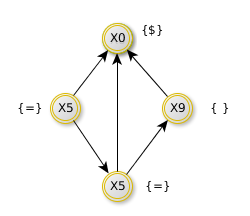
\includegraphics[scale=0.6]{Chapters/Img/l01_01.png}\\
\end{center} 

\begin{tabular}{l}
	$x_0 = \{ \$ \}$\\
	$x_5 = \{ =, \$ \}$\\
	$x_6 = \{ =, \$ \}$\\
	$x_9 = \{ =, \$ \}$\\
\end{tabular}

\section{Algoritmo}
Algoritmo utilizzato da yacc (su dragonbook)
Uso LR0, per ogni item dentro uno stato faccio una chiusura virtuale LR1
Faccio un nuovo grafo e ...

Identifica look ahead generati e propagati, poi fa un grafo e associa ad ogni nodo il look ahead generato

\begin{center}
	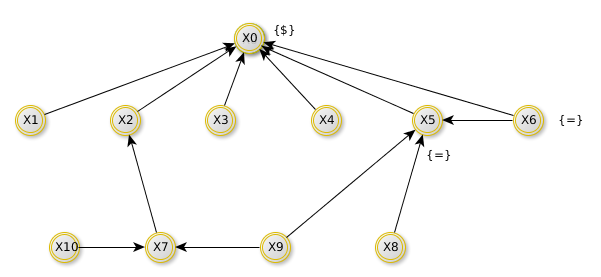
\includegraphics[scale=0.6]{Chapters/Img/l01_02.png}\\
\end{center} 

\begin{tcolorbox}\begin{center}
	Kernel(P) L'insiseme dei kernel item dentro P, proj(P) L'inisieme degli item LR(0) contenuti in P
\end{center}\end{tcolorbox}

\section{Costruzione automa simbolico}
\begin{lstlisting}
	x_0 = new Var()
	vars = {x_0}
	P_0 = closure_1( { [s' -> .s, {x_0} ] } ) //stato iniziale automa
	inizializzare Queue con x_0 = {$}
	States = {P_0}
	porre P_0 come unmarked
	while(c'e' uno stato non marcato P in States){
		marcare P
		foreach(y in V){
			Tmp = emptySet
			foreach([A -> alpha.y beta, delta] <- P){
				aggiungere [A -> alpha.y beta, delta] a Tmp
				if(Tmp != emptySet){
					if( lo stato targhet non e' ancora stato collezionato){
						aggiungere a States una versione simbolica del targhet e aggiungere a Queue una equazione per kernel item in Tmp
					} else {
						raffinare le equazioni delle variabili associate ai kernel item del target
					}
				}
			}
		}
	}
\end{lstlisting}


%\section{Grammatiche Attribute}
SDD (Syntax Directed Definition)
SDT (Syntax Directed Translation)

Aggiungo alla grammatica degli attributi e delle regole per quest'utlimi.
(Desc Calculator) posso computare valori associati ad espressioni aritmetiche.

%%%%%%%%%%%%%%%%%%%%%%%%%%%%%%%%%%%%%%%%%%%%%%%%%%%%%%%%%%%%%%%%%%%%%%%%%%%%
\subsection{Esempio}
\begin{tabular}{l}
	$E \rightarrow E + T | T$\\
	$T \rightarrow T * F | F$\\
	$F \rightarrow (E) | id$\\
\end{tabular}

Associo attributi ai terminali e non terminali, che recupero dall'analisi lessicale.

\begin{center}
	$3 + 4 * 5$ \\
	\Tree[. E [.E [.T [.F [.id (3) ] ] ] ] + [.T [.T [.F [.id (4) ] ] ] * [.F [.id (5) ] ] ] ]\\
\end{center}


Faccio visita postorder dell'albero (Bottom Up), associo i valori degli attributi a id, poi a F, poi risalgo a T. Quando sonon in T * F, T=4, F=5;
Quindi risolvo 4*5 che assegno come attributo al nodo padre T.

\begin{tcolorbox}\begin{center}
	\textbf{E.val} per indicare l'attributo della E.
\end{center}\end{tcolorbox}

\begin{tabular}{ll}
	$ \$\$ $ 	& Il driver\\
	$ \$ 1 $	& Primo elemento della produzione\\
\end{tabular}	 

$E_1 \rightarrow E_2 + T$ $\{ E_1.val = E_2.val + T.val \} $ \textbf{azione semantica} \\
$E \rightarrow T$ $\{ E.val = T.val \} $ \\
$T_1 \rightarrow T_2 * F $ $\{ T_1.val = T_2.val + F.val \} $ \\
$T \rightarrow F $ $ T.val = F.val $ \\
$F \rightarrow (E) $ $\{ F.val = E.val \} $ \\
$F \rightarrow id $ $\{ F.val = lexval(id) \} $ \\

Abstract Syntax Tree (albero derivazione \lq\lq ristretto\rq\rq )
\Tree[.+ $id_3$ [.* $id_4$ $id_5$ ] ]

\subsection{Attributi sintetizzati}
$A \rightarrow \alpha $ A.a definito come una funzione degli attributi dei terminali e non terminali in $\alpha $.
Gli attributi dei terminali derivano dall'analisi lessicale.

\subsection{Esempio, dichiarazione variabili}
\begin{lstlisting}
	int pippo, pluto, paperino;
\end{lstlisting}

$D \rightarrow TL$ $\{ L.i = T.t \} $\\
$T \rightarrow int$ $\{ T.t = integer\} $\\
$T \rightarrow float$ $\{ T.t = float \} $\\
$L_1 \rightarrow L_2,\ id$ $\{ L_2.i = L_1.i,\ addType(lex(id), L_1.i) \} $\\
$L \rightarrow id$ $\{ addType(lex(id)),\ L_i) \} $\\

\Tree[.D [.T int ] [.L [.L [.L [.id (pluto) ] ] , [.id (pippo) ] ] , [.id (paperino) ] ] ]

\begin{center}
	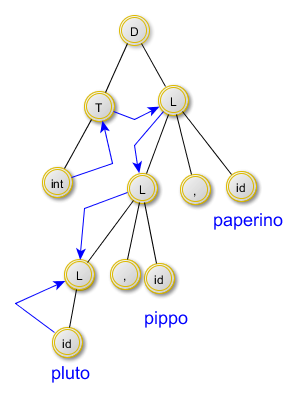
\includegraphics[scale=0.5]{Chapters/Img/l02_01.png}\\
\end{center} 

Gli attributi ereditati sono funzione degli attributi di siblings e del padre (driver della produzione).

\subsection{Example}
$S \rightarrow Number$\\
$Number \rightarrow o Digits$ serie di cifre in ottali (o)\\
$Number \rightarrow Digits d$\\
$Digits \rightarrow d$\\

\Tree[.N o [.Digits [.(...) d ] d ] ]

Gira l'albero!
$ S \rightarrow Digits $\\
$ Digits_1 \rightarrow Digits_2 d $ $\{ Digits_1.val = Digits_2 * Dg.tg_2.base + "d" \}$\\
$ Digits \rightarrow d $ $\{ Digit.base = 10; Digit.val = "d" \}$\\
$ Digits \rightarrow od $ $\{ Digit.base = 8; Digit.val = "d" \}$\\

Supponiamo per assurdo che sia LALR.
\end{document}